%%%%%%%%%%%%%%%%%%%%%%%%%%%%%%%%%%%%%%%%%%%%%%%%%%%%%%
% A Beamer template for University of Wollongong     %
% Based on THU beamer theme                          %
% Author: Qiuyu Lu                                   %
% Date: July 2024                                    %
% LPPL Licensed.                                     %
%%%%%%%%%%%%%%%%%%%%%%%%%%%%%%%%%%%%%%%%%%%%%%%%%%%%%%
% Customized for Sharif University of Technology     %
%%%%%%%%%%%%%%%%%%%%%%%%%%%%%%%%%%%%%%%%%%%%%%%%%%%%%%


\documentclass[serif, aspectratio=169]{beamer}
\usepackage{pgfplots} % Required for plotting
\pgfplotsset{compat=1.17} % Compatibility level
%\documentclass[serif]{beamer}  % for 4:3 ratio
\usepackage[T1]{fontenc} 
\usepackage{fourier} % see "http://faq.ktug.org/wiki/uploads/MathFonts.pdf" for other options
\usepackage{hyperref}
\usepackage{latexsym,amsmath,xcolor,multicol,booktabs,calligra}
\usepackage{graphicx,pstricks,listings,stackengine}
\usepackage{lipsum}
\usepackage{tikz}
\usepackage{subfigure}
\usetikzlibrary{positioning, arrows.meta}

\author{Ali Sharifi-Zarchi}
\title{Machine Learning (CE 40477)}
\subtitle{Fall 2024}
\institute{
    CE Department \\
    Sharif University of Technology
}
%\date{\small \today}
% \usepackage{UoWstyle}
\usepackage{SUTstyle}

% defs
\def\cmd#1{\texttt{\color{red}\footnotesize $\backslash$#1}}
\def\env#1{\texttt{\color{blue}\footnotesize #1}}
\definecolor{deepblue}{rgb}{0,0,0.5}
\definecolor{deepred}{RGB}{153,0,0}
\definecolor{deepgreen}{rgb}{0,0.5,0}
\definecolor{halfgray}{gray}{0.55}

\lstset{
    basicstyle=\ttfamily\small,
    keywordstyle=\bfseries\color{deepblue},
    emphstyle=\ttfamily\color{deepred},    % Custom highlighting style
    stringstyle=\color{deepgreen},
    numbers=left,
    numberstyle=\small\color{halfgray},
    rulesepcolor=\color{red!20!green!20!blue!20},
    frame=shadowbox,
}


\begin{document}

\begin{frame}
    \titlepage
    \vspace*{-0.6cm}
    \begin{figure}[htpb]
        \begin{center}
            
\includegraphics[keepaspectratio, scale=0.25]{pic/sharif-main-logo.png}
        \end{center}
    \end{figure}
\end{frame}

\begin{frame}    
\tableofcontents[sectionstyle=show,
subsectionstyle=show/shaded/hide,
subsubsectionstyle=show/shaded/hide]
\end{frame}


\section{Batch Normalization}


\subsection{Why Batch Normalization?}

\begin{frame}{Why Batch Normalization?}

    \textcolor{blue}{\textbf{Problem: Internal Covariate Shift}}

\begin{itemize}

    \item What does it mean, in simple terms?
    \item Let’s say that we want to train a model and the ideal target output function that the model needs to learn is as below:

    \begin{figure}
        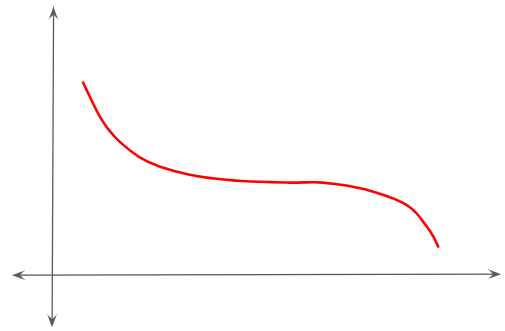
\includegraphics[width=0.45\textwidth]{pic/ICS-1.png}
        % \caption{Target function \href{https://ketanhdoshi.github.io/assets/images/BatchNorm/ICS-1.png}{\textcolor{orange}{\textbf{Source}}}}
        \label{fig:Target_function}
    \end{figure}

        \vfill
    \begin{tikzpicture}[remember picture,overlay]
        \node[anchor=south west, xshift=0.15cm, yshift=0.22cm] at (current page.south west) {
            \tiny Figure adapted from Ketan Doshi. Batch Normalization: A Comprehensive Blog
        };
    \end{tikzpicture}

\end{itemize}

\end{frame}

\begin{frame}{Problem: Internal Covariate Shift}

\begin{itemize}

    \item Suppose that the training data values input to the model cover only a part of the range of output values. Therefore, the model can only learn a subset of the target function.

    \begin{figure}
        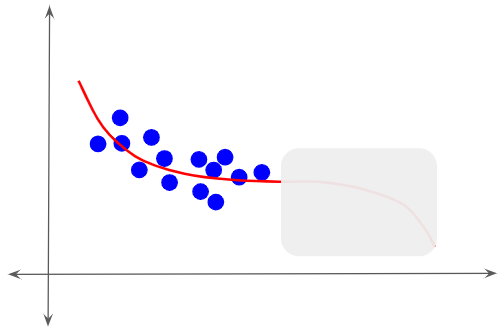
\includegraphics[width=0.45\textwidth]{pic/ICS-2.png}
        % \caption{Training data distribution \href{https://ketanhdoshi.github.io/assets/images/BatchNorm/ICS-2.png}{\textcolor{orange}{\textbf{Source}}}}
        \label{fig:Training_data_distribution}
    \end{figure}

    \vfill
    \begin{tikzpicture}[remember picture,overlay]
        \node[anchor=south west, xshift=0.1cm, yshift=0.22cm] at (current page.south west) {
            \tiny Figure adapted from Ketan Doshi. Batch Normalization: A Comprehensive Blog
        };
    \end{tikzpicture}

\end{itemize}

\end{frame}

\begin{frame}{Problem: Internal Covariate Shift}

\begin{itemize}

    \item The model has no idea about the rest of the target curve. It could be anything.

    \begin{figure}
        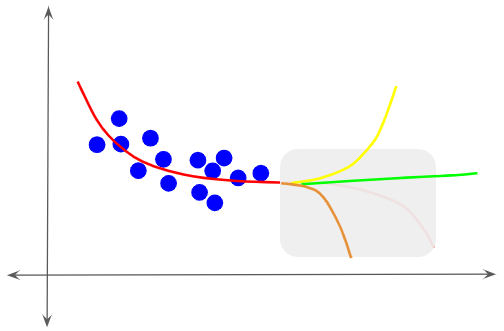
\includegraphics[width=0.45\textwidth]{pic/ICS-3.png}
        % \caption{Rest of the target curve \href{https://ketanhdoshi.github.io/assets/images/BatchNorm/ICS-3.png}{\textcolor{orange}{\textbf{Source}}}}
        \label{fig:Rest_Curve}
    \end{figure}

    \vfill
    \begin{tikzpicture}[remember picture,overlay]
        \node[anchor=south west, xshift=0.1cm, yshift=0.22cm] at (current page.south west) {
            \tiny Figure adapted from Ketan Doshi. Batch Normalization: A Comprehensive Blog
        };
    \end{tikzpicture}

\end{itemize}

\end{frame}

\begin{frame}{Problem: Internal Covariate Shift}

\begin{itemize}

    \item Suppose we feed the model to the testing data as below.
    \item This has a very different distribution from the data that the model was initially trained with.
    \item The model cannot simply generalize its predictions for this new data.

    \begin{figure}
        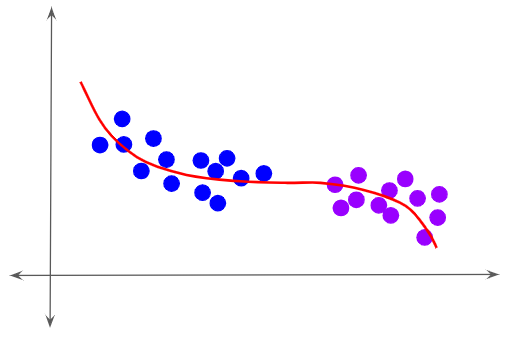
\includegraphics[width=0.4\textwidth]{pic/ICS-4.png}
        % \caption{The rest of the data has different distribution \href{https://ketanhdoshi.github.io/assets/images/BatchNorm/ICS-4.png}{\textcolor{orange}{\textbf{Source}}}}
        \label{fig:Rest_data_distribution}
    \end{figure}

    \vfill
    \begin{tikzpicture}[remember picture,overlay]
        \node[anchor=south west, xshift=0.1cm, yshift=0.22cm] at (current page.south west) {
            \tiny Figure adapted from Ketan Doshi. Batch Normalization: A Comprehensive Blog
        };
    \end{tikzpicture}

\end{itemize}

\end{frame}

\begin{frame}{Problem: Internal Covariate Shift}
    
\begin{itemize}
    \item Covariate Shift occurs when \textbf{the model is fed data with a different distribution than what it was previously trained with}, even though that new data still conforms to the same target function.

    \item For the model to figure out how to adapt to this new data, it has to re-learn some of its target output functions.
    \item \textbf{This slows down the training process.}
    
\end{itemize}

\end{frame}

\begin{frame}{Problem: Internal Covariate Shift}
	
	\textcolor{blue}{\textbf{What happens inside Deep Network Layers?}}
	
	\begin{itemize}
		
		\item Consider what happens when training a deep network: As we update the weights of earlier layers, the data distribution in the deeper layer keeps shifting.
		
		\item Deeper layers see new and varying patterns every time we update the weights in previous layers.
		
		\begin{figure}
			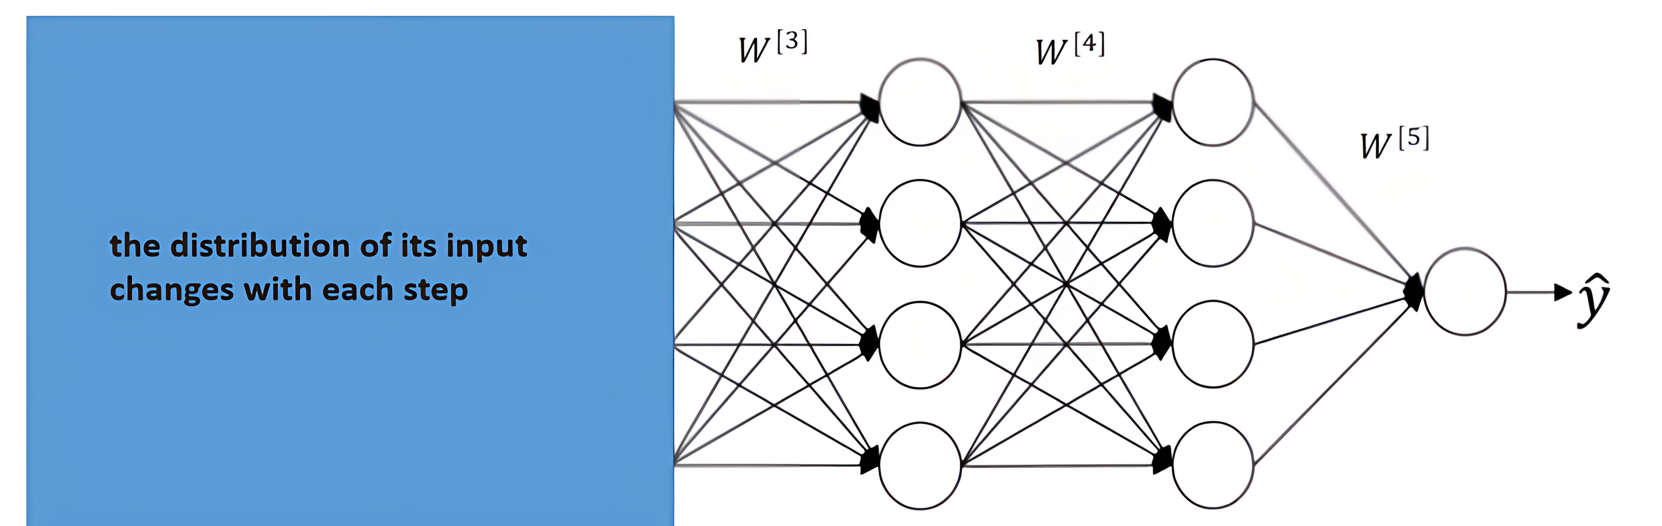
\includegraphics[width=0.8\textwidth]{pic/change-distribution.png}
			\label{fig:change_distribution}
		\end{figure}
		
		\vfill
		\begin{tikzpicture}[remember picture,overlay]
			\node[anchor=south west, xshift=0.1cm, yshift=0.22cm] at (current page.south west) {
				\tiny Figure adapted from Andrew Ng, Deep Learning Specialization Course
			};
		\end{tikzpicture}
		
	\end{itemize}
	
\end{frame}

\begin{frame}{Problem: Internal Covariate Shift}
	
	\textcolor{blue}{\textbf{What happens inside Deep Network Layers?}}
	
	\begin{itemize}
		
		\item The network must keep readjusting, which makes the learning process slower and more challenging.
		\item \textbf{In other words:} The network is constantly “re-learning” how to make predictions because the data it sees is never consistent.
		
	\end{itemize}
	
\end{frame}

\begin{frame}{Batch Normalization Solution}

    \begin{itemize}
        \item \textbf{Goal:} Normalize inputs so that the mean is near 0 and the variance is close to 1.
        \item \textbf{How it helps:} Stabilizes learning, allowing for higher learning-rates and faster convergence.
    \end{itemize}

\end{frame}

%\begin{frame}{Batch Normalization Solution}
%	
%	\begin{itemize}
%		\item What’s the link between Batch Normalization and this picture?
%	\end{itemize}
%	
%	\begin{figure}
%		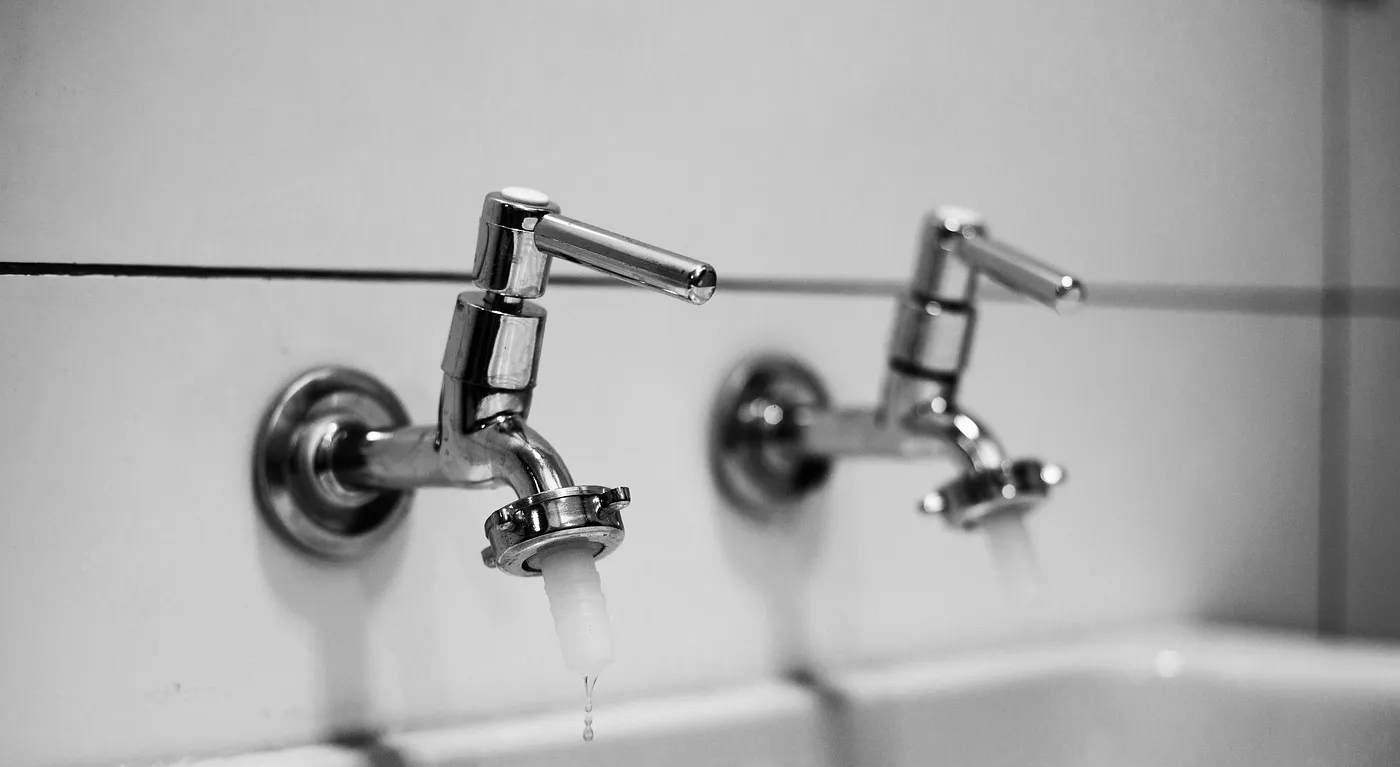
\includegraphics[width=0.6\textwidth]{pic/BN-Q.png}
%		\label{fig:BN-Q}
%	\end{figure}
%	
%	\vfill
%	\begin{tikzpicture}[remember picture,overlay]
%		\node[anchor=south west, xshift=0.1cm, yshift=0.22cm] at (current page.south west) {
%			\tiny Figure adapted from Danilo Alvesd on Unsplash
%		};
%	\end{tikzpicture}
%	
%\end{frame}
%
%\begin{frame}{Batch Normalization Solution}
%	
%	\begin{itemize}
%		\item The two faucets represent two separate control mechanisms—like the mean and variance adjustments in Batch Normalization—working together to keep the flow (activations) at an optimal, consistent range, preventing extreme values (too hot or too cold) that can disrupt learning.
%	\end{itemize}
%	
%		\begin{figure}
%		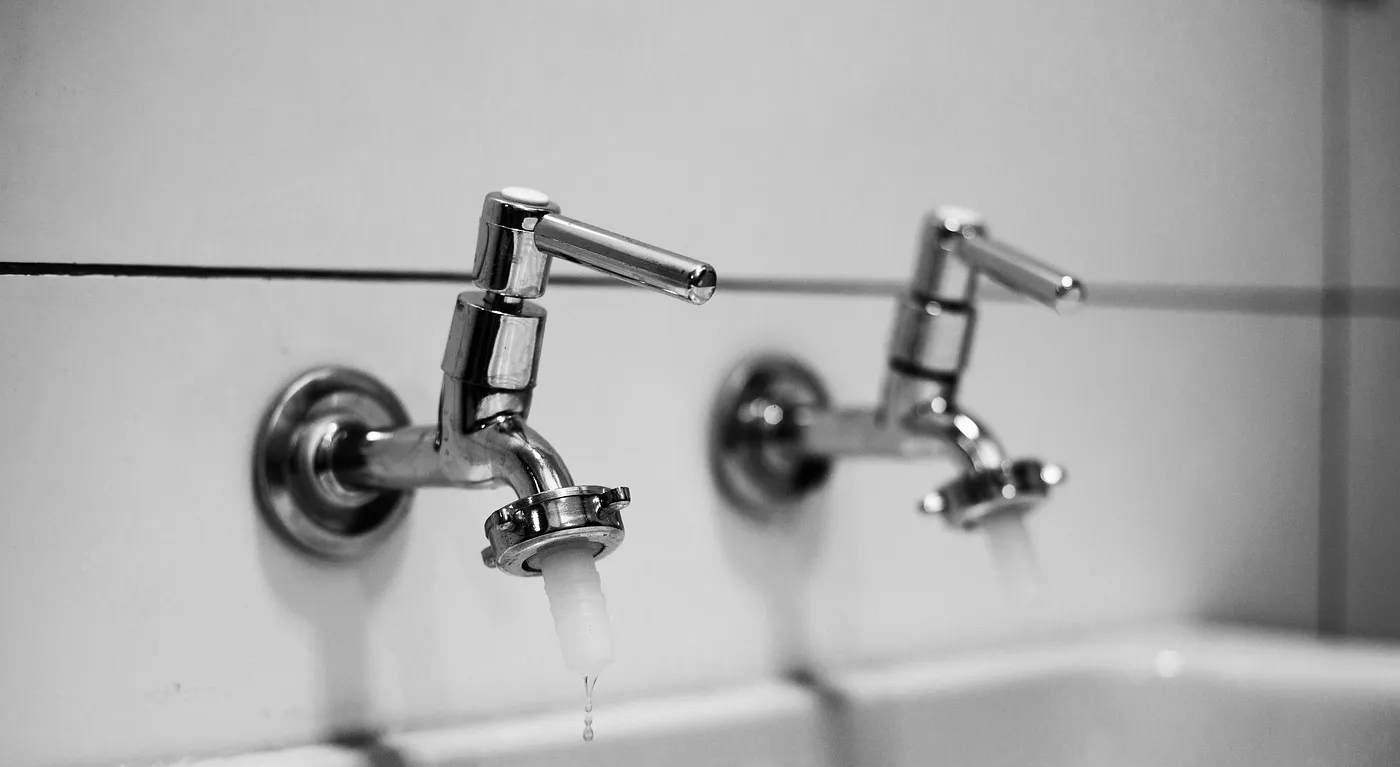
\includegraphics[width=0.4\textwidth]{pic/BN-Q.png}
%		\label{fig:BN-Q2}
%	\end{figure}
%	
%	\vfill
%	\begin{tikzpicture}[remember picture,overlay]
%		\node[anchor=south west, xshift=0.1cm, yshift=0.22cm] at (current page.south west) {
%			\tiny Figure adapted from Danilo Alvesd on Unsplash
%		};
%	\end{tikzpicture}
%	
%\end{frame}

\subsection{How Batch Normalization Works}

\begin{frame}{How Batch Normalization Works}

    \textcolor{blue}{\textbf{Process Overview}}
    
    \begin{itemize}

        \item  For each mini-batch during training, batch normalization normalizes the inputs to a layer by adjusting their mean and variance.

    \end{itemize}
\end{frame}

% Frame 1: Steps 1 and 2
\begin{frame}{How Batch Normalization Works}
\textcolor{blue}{\textbf{Steps in Batch Normalization}}
\begin{enumerate}
    \item \textbf{Compute the Mean and Variance} 
          \newline
          For a given mini-batch, compute the mean $\mu_B$ and variance $\sigma_B^2$ of the inputs:

          \[
           \mu_B = \frac{1}{m} \sum_{i=1}^{m} x_i, \quad \sigma_B^2 = \frac{1}{m} \sum_{i=1}^{m} (x_i - \mu_B)^2
          \]
    \item \textbf{Normalize the Inputs}
    \newline
    Subtract the mean and divide by the standard deviation to get normalized activations:
    \[
    \hat{x}_i = \frac{x_i - \mu_B}{\sqrt{\sigma_B^2 + \epsilon}}
    \]
    where $\epsilon$ is a small constant added for numerical stability.
\end{enumerate}
\end{frame}

% Frame 2: Step 3
\begin{frame}{How Batch Normalization Works (Continued)}
\textcolor{blue}{\textbf{Steps in Batch Normalization}}
\begin{enumerate}
    \setcounter{enumi}{2} % Set the counter to continue from step 3
    \item \textbf{Scale and Shift}
    \newline
    After normalization, introduce learnable parameters $\gamma$ and $\beta$ that allow the model to scale and shift the normalized output:

    \[
        y_i = \gamma \hat{x}_i + \beta
    \]
    This allows that the model to recover the original data distribution if necessary.
\end{enumerate}
\end{frame}

\begin{frame}{Smoothing the optimization space}
	
	\begin{figure}
		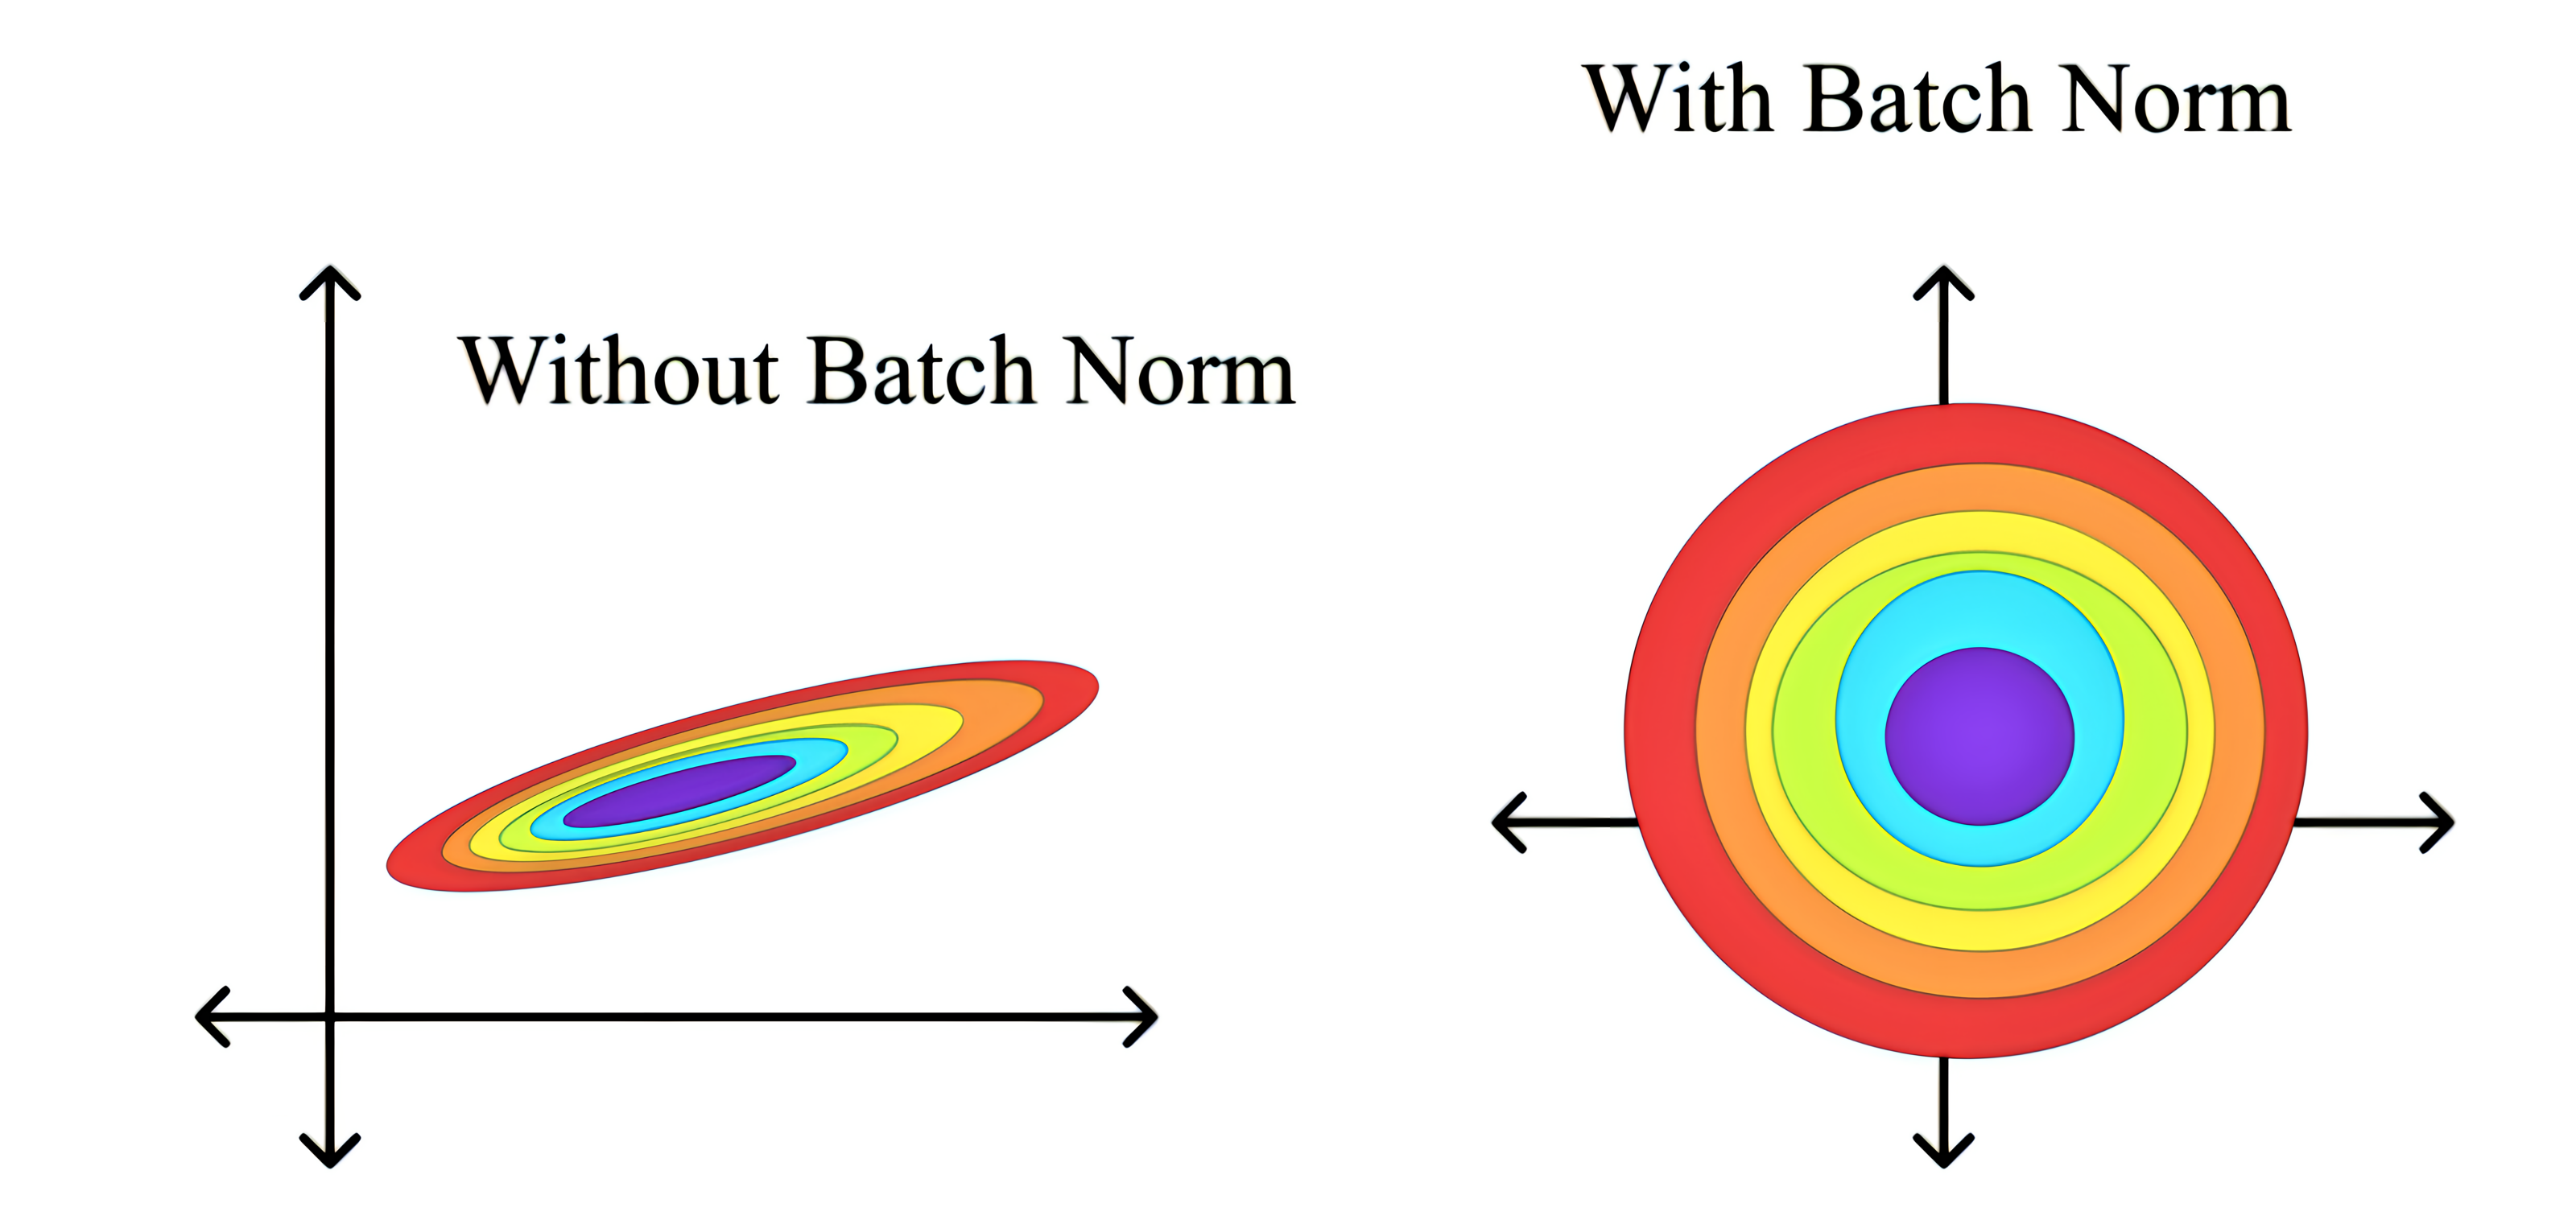
\includegraphics[width=0.85\textwidth]{pic/BatchNorm_Effect.png}
		% \caption{Using Batch Normalization causes the optimization space to become smoother. \href{https://www.linkedin.com/pulse/ways-improve-your-deep-learning-model-batch-adam-albuquerque-lima}{\textcolor{orange}{\textbf{Source}}}}
		\label{fig:BN_Effect1}
	\end{figure}
	
	\vfill
	\begin{tikzpicture}[remember picture,overlay]
		\node[anchor=south west, xshift=0.1cm, yshift=0.22cm] at (current page.south west) {
			\tiny Figure adapted from Gustavo Albuquerque Lima. Ways to Improve Your Deep Learning Model - Batch Normalization and Adam: A Short Course
		};
	\end{tikzpicture}
	
\end{frame}

\begin{frame}{Effect of Batch Normalization}
	
	\begin{itemize}
		\item Batch Normalization helps the network train faster and achieve higher accuracy.
		\item Batch Normalization \textbf{stabilizes the distribution} and reduces the internal covariate shift.
	\end{itemize}
	
	\begin{figure}
		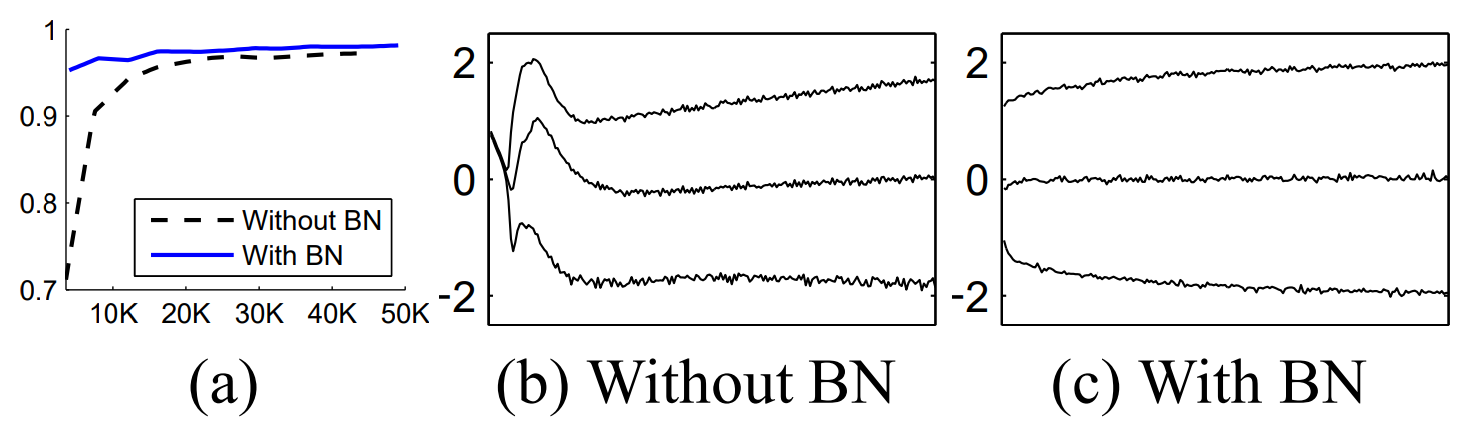
\includegraphics[width=0.3\textwidth]{pic/BN.png}
		\label{fig:BN_Effect}
	\end{figure}
	
	\begin{itemize}
		\item The test accuracy of the \texttt{MNIST} network trained with and without Batch Normalization, vs the number of training steps.
	\end{itemize}
	
	    \vfill
	\begin{tikzpicture}[remember picture,overlay]
		\node[anchor=south west, xshift=0.1cm, yshift=0.22cm] at (current page.south west) {
			\tiny Figure adapted from Johan Bjorck et al. Understanding Batch Normalization Paper, https://doi.org/10.48550/arXiv.1806.02375
		};
	\end{tikzpicture}

	
\end{frame}

\begin{frame}{Effect of Batch Normalization}
	
	\begin{figure}[h!]
		\centering
		\begin{minipage}{0.44\textwidth}
			\centering
			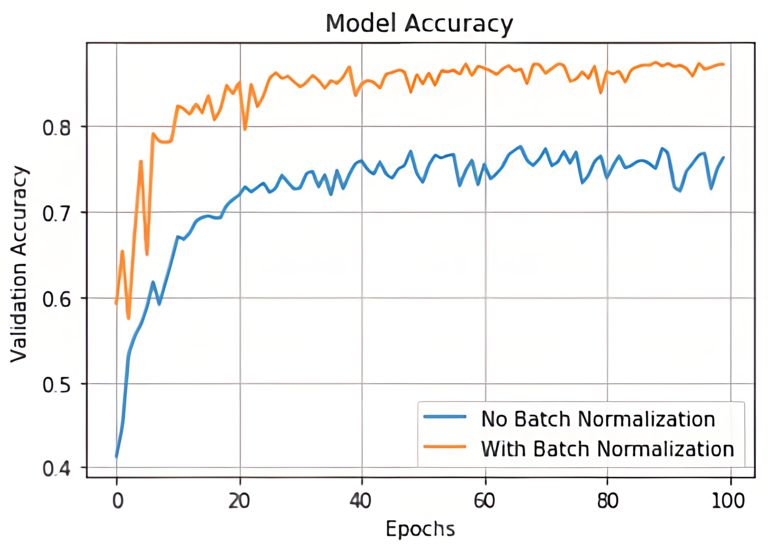
\includegraphics[width=\linewidth]{pic/ModelAccuracy.png}
			\label{fig:fig1}
		\end{minipage} \hfill
%		\hspace{0.02\textwidth} % Space before the line
%		\vrule width 0.5pt % Thickness of the line
%		\hspace{0.02\textwidth} % Space after the line
		\begin{minipage}{0.5\textwidth}
			\centering
			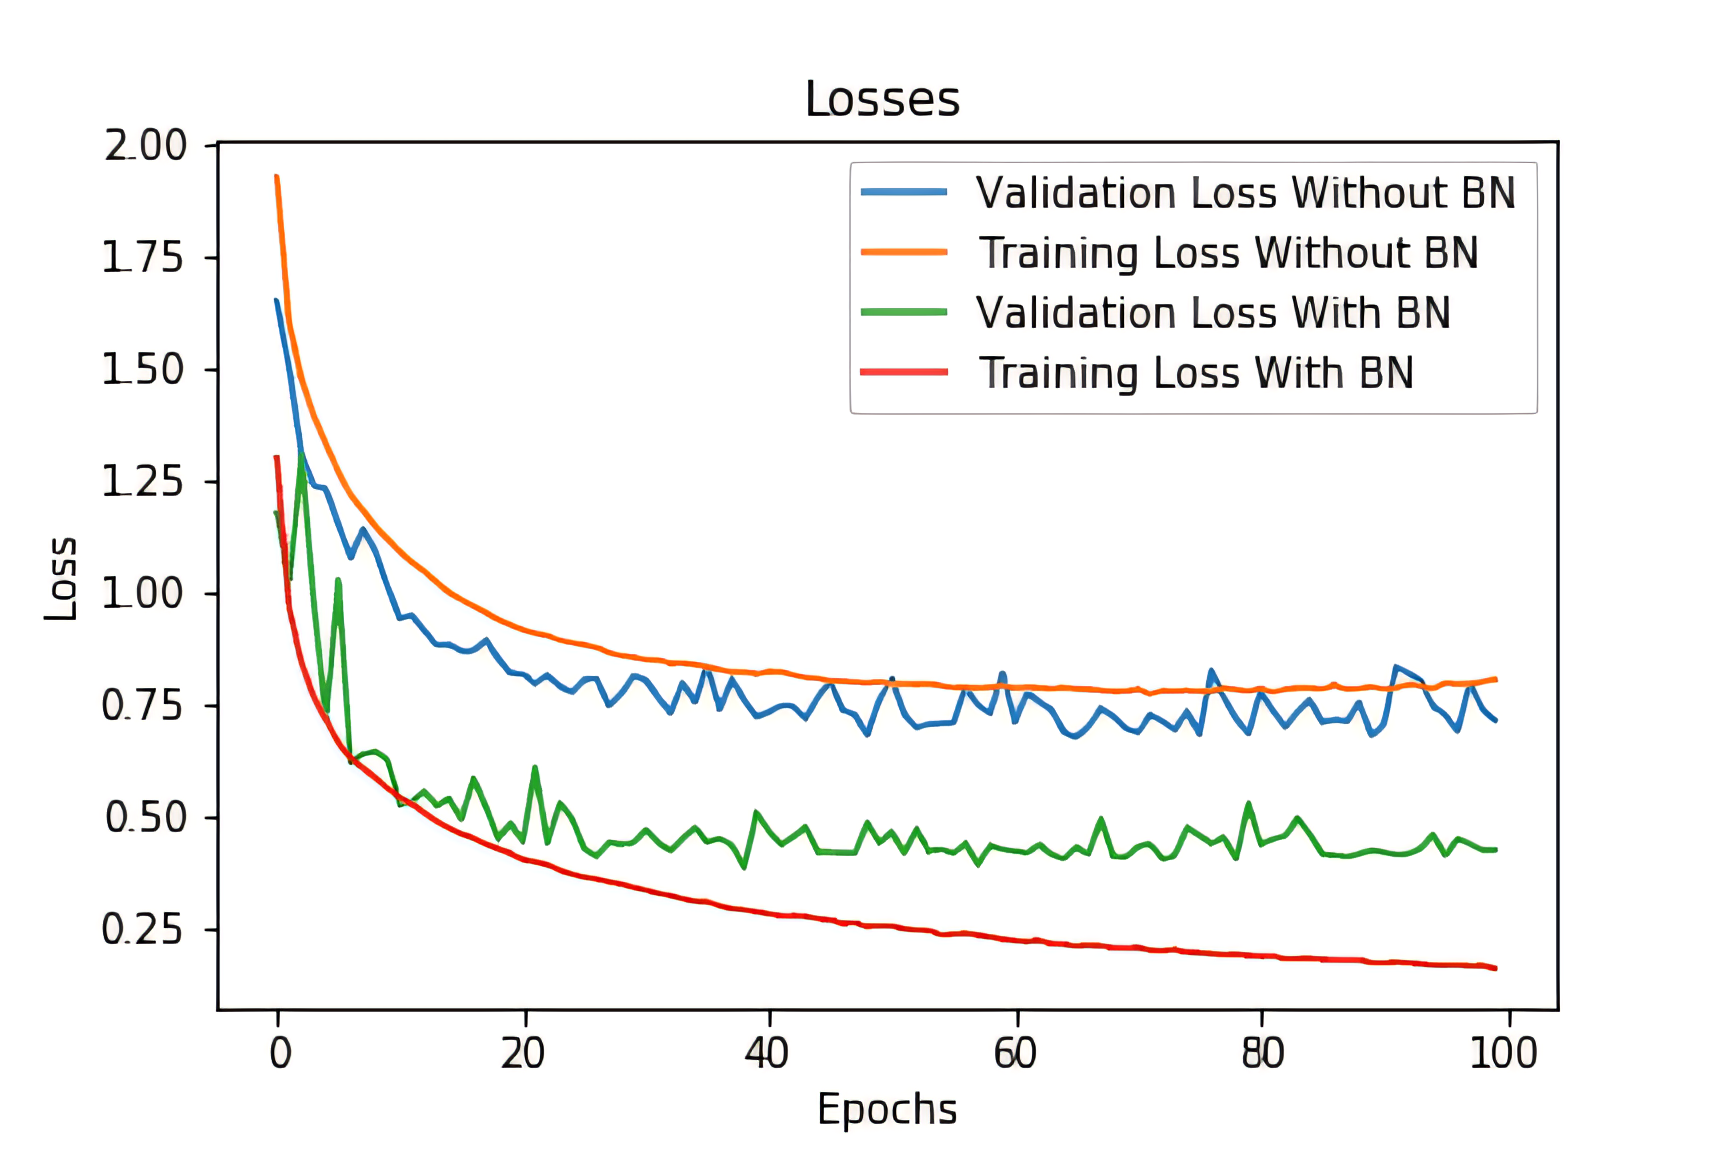
\includegraphics[width=\linewidth]{pic/val_loss.png}
			\label{fig:fig2}
		\end{minipage}
	\end{figure}
	
	\vfill
	\begin{tikzpicture}[remember picture,overlay]
		\node[anchor=south west, xshift=0.1cm, yshift=0.22cm] at (current page.south west) {
			\tiny Figure adapted from Sunita Nayak, Batch Normalization in Deep Networks on LearnOpenCV
		};
	\end{tikzpicture}
	
	
\end{frame}


\begin{frame}{Effect of Batch Normalization on Gradients}
        \begin{figure}
        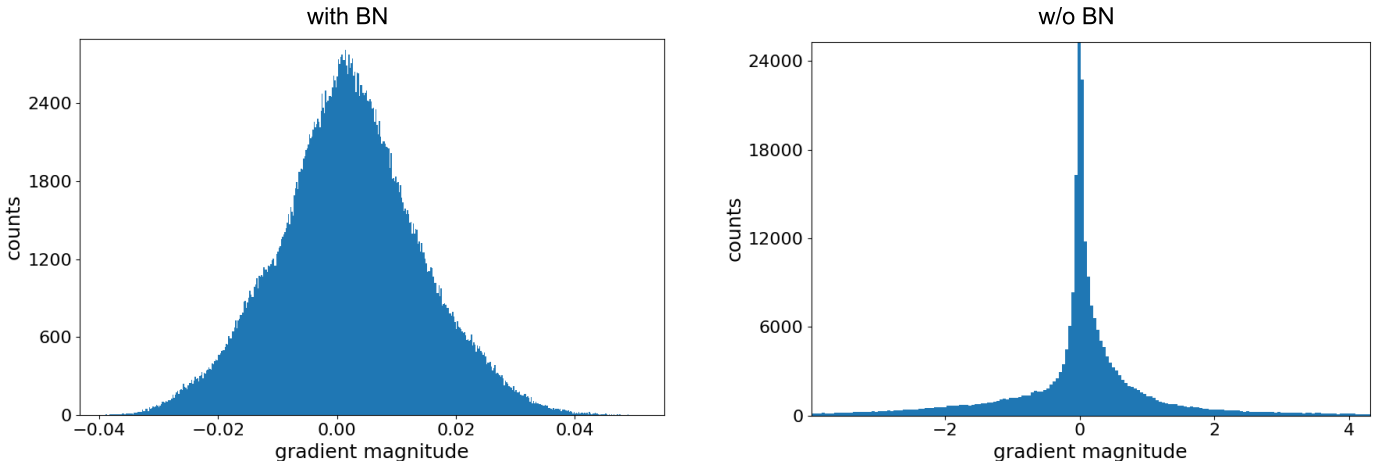
\includegraphics[width=0.9\textwidth]{pic/BN_Grad_Dist.png}
        % \caption{Gradient magnitudes at initialization for layer 55 of a network with and without Batch Normalization. \href{https://doi.org/10.48550/arXiv.1806.02375}{\textcolor{orange}{\textbf{Source}}}}
        \label{fig:BN_Dist}
    \end{figure}

    \vfill
    \begin{tikzpicture}[remember picture,overlay]
        \node[anchor=south west, xshift=0.1cm, yshift=0.22cm] at (current page.south west) {
            \tiny Figure adapted from Johan Bjorck et al. Understanding Batch Normalization Paper, https://doi.org/10.48550/arXiv.1806.02375
        };
    \end{tikzpicture}
    
\end{frame}

%\begin{frame}{Effect of Batch Normalization on Gradients}
%        \begin{figure}
%        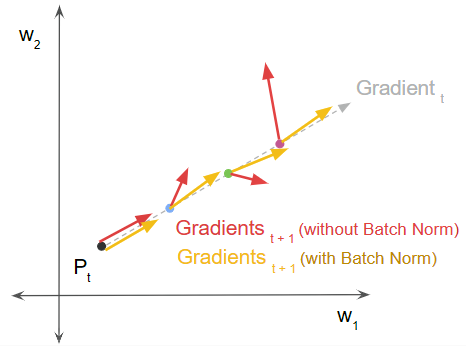
\includegraphics[width=0.55\textwidth]{pic/Smooth.png}
%        % \caption{Gradients with Batch Norm are smoother. \href{https://ketanhdoshi.github.io/Batch-Norm-Why/}{\textcolor{orange}{\textbf{Source}}}}
%        \label{fig:Smooth}
%    \end{figure}
%
%    \vfill
%    \begin{tikzpicture}[remember picture,overlay]
%        \node[anchor=south west, xshift=0.1cm, yshift=0.22cm] at (current page.south west) {
%            \tiny Figure adapted from Ketan Doshi. Batch Normalization: A Comprehensive Blog
%        };
%    \end{tikzpicture}
%\end{frame}

\begin{frame}
    \frametitle{Effect of Batch Normalization on Gradients}

    The main benefit of batch normalization is that it reduces the dependency of gradient on the scale of input and parameters:

    \begin{equation}
        \frac{\partial \mathcal{L}}{\partial x} = \frac{\partial \mathcal{L}}{\partial y} \cdot \frac{\partial y}{\partial \hat{x}} \cdot \frac{\partial \hat{x}}{\partial x}
    \end{equation}

    Where:
    \begin{itemize}
        \item \centering \(\frac{\partial y}{\partial \hat{x}} = \gamma\) \\
        \item \(\frac{\partial \hat{x}}{\partial x} = \frac{1}{\sqrt{\sigma_{\mathcal{B}}^2 + \epsilon}}\)
    \end{itemize}

    Thus, the gradient becomes:
    \begin{equation}
        \frac{\partial \mathcal{L}}{\partial x} = \frac{\gamma}{\sqrt{\sigma_{\mathcal{B}}^2 + \epsilon}} \cdot \frac{\partial \mathcal{L}}{\partial y}
    \end{equation}
\end{frame}





%\begin{frame}
%    \frametitle{Loss Landscape is not Smooth in Typical Neural Networks}
%    \begin{figure}
%        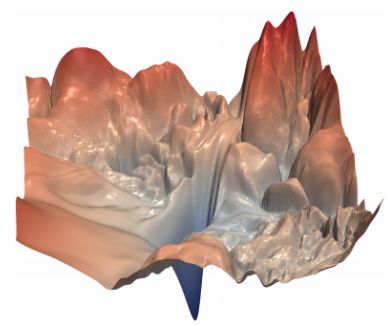
\includegraphics[width=0.45\textwidth]{pic/Landscape-1.png}
%        % \caption{A neural network loss-landscape. \href{https://arxiv.org/pdf/1712.09913.pdf}{\textcolor{orange}{\textbf{Source}}}}
%        \label{fig:Loss_Landscape}
%    \end{figure}
%
%        \vfill
%    \begin{tikzpicture}[remember picture,overlay]
%        \node[anchor=south west, xshift=0.1cm, yshift=0.22cm] at (current page.south west) {
%            \tiny Figure adapted from Hao Li et al. Visualizing the Loss Landscape of Neural Nets, https://arxiv.org/pdf/1712.09913.pdf
%        };
%    \end{tikzpicture}
%\end{frame}

\begin{frame}
    \frametitle{How Batch Normalization Smooth the  Loss Landscape}

    The smoothing effect of batch normalization can be understood by observing how it constrains the gradient magnitudes. The expression shows that:
    \begin{equation}
        \frac{\partial \mathcal{L}}{\partial x} \text{ is scaled by } \frac{1}{\sqrt{\sigma_{\mathcal{B}}^2 + \epsilon}}
    \end{equation}

    This consistent scaling results in a smooth loss landscape because:
    \begin{itemize}
        \item It stabilizes the gradient flow, ensuring controlled optimization step sizes.
        \item Reduces the risk of large oscillations or abrupt changes in the loss landscape.
        \item Makes the optimization process less likely to be trapped in local minima or saddle points.
    \end{itemize}
\end{frame}


\subsection{Batch Normalization Pros \& Cons}

\begin{frame}{Batch Normalization Pros}

    \textbf{Pros}
    
    \begin{itemize}

        \item \textbf{Faster Convergence:}  Empirical results support that models with batch normalization converge faster and achieve higher accuracy, even with \textbf{higher learning rates}.
        \item \textbf{Reduced Sensitivity to  Weight Initialization:} Mitigate the dependency on careful weight initialization.
        \item \textbf{Acts as Regularization:} Batch normalization can help reduce overfitting.
        \item \textbf{Reduces Vanishing/Exploding Gradients:} Maintains stable gradients throughout deep networks.


    \end{itemize}
\end{frame}


\begin{frame}{Batch Normalization During Inference Mode}
	
	\textcolor{blue}{\textbf{Inference Mode:}}
	
	\begin{itemize}
		
		\item During inference (when predicting new data), batch statistics (mean and variance) are replaced with moving averages collected during training.
		
	\end{itemize}
\end{frame}

\begin{frame}{Batch Normalization Pros}

    \textcolor{blue}{\textbf{Why Using Batch Normalization Reduces Sensitivity to Weight Initialization?}}

    \begin{figure}[h]
        \centering
        \subfigure[]{
            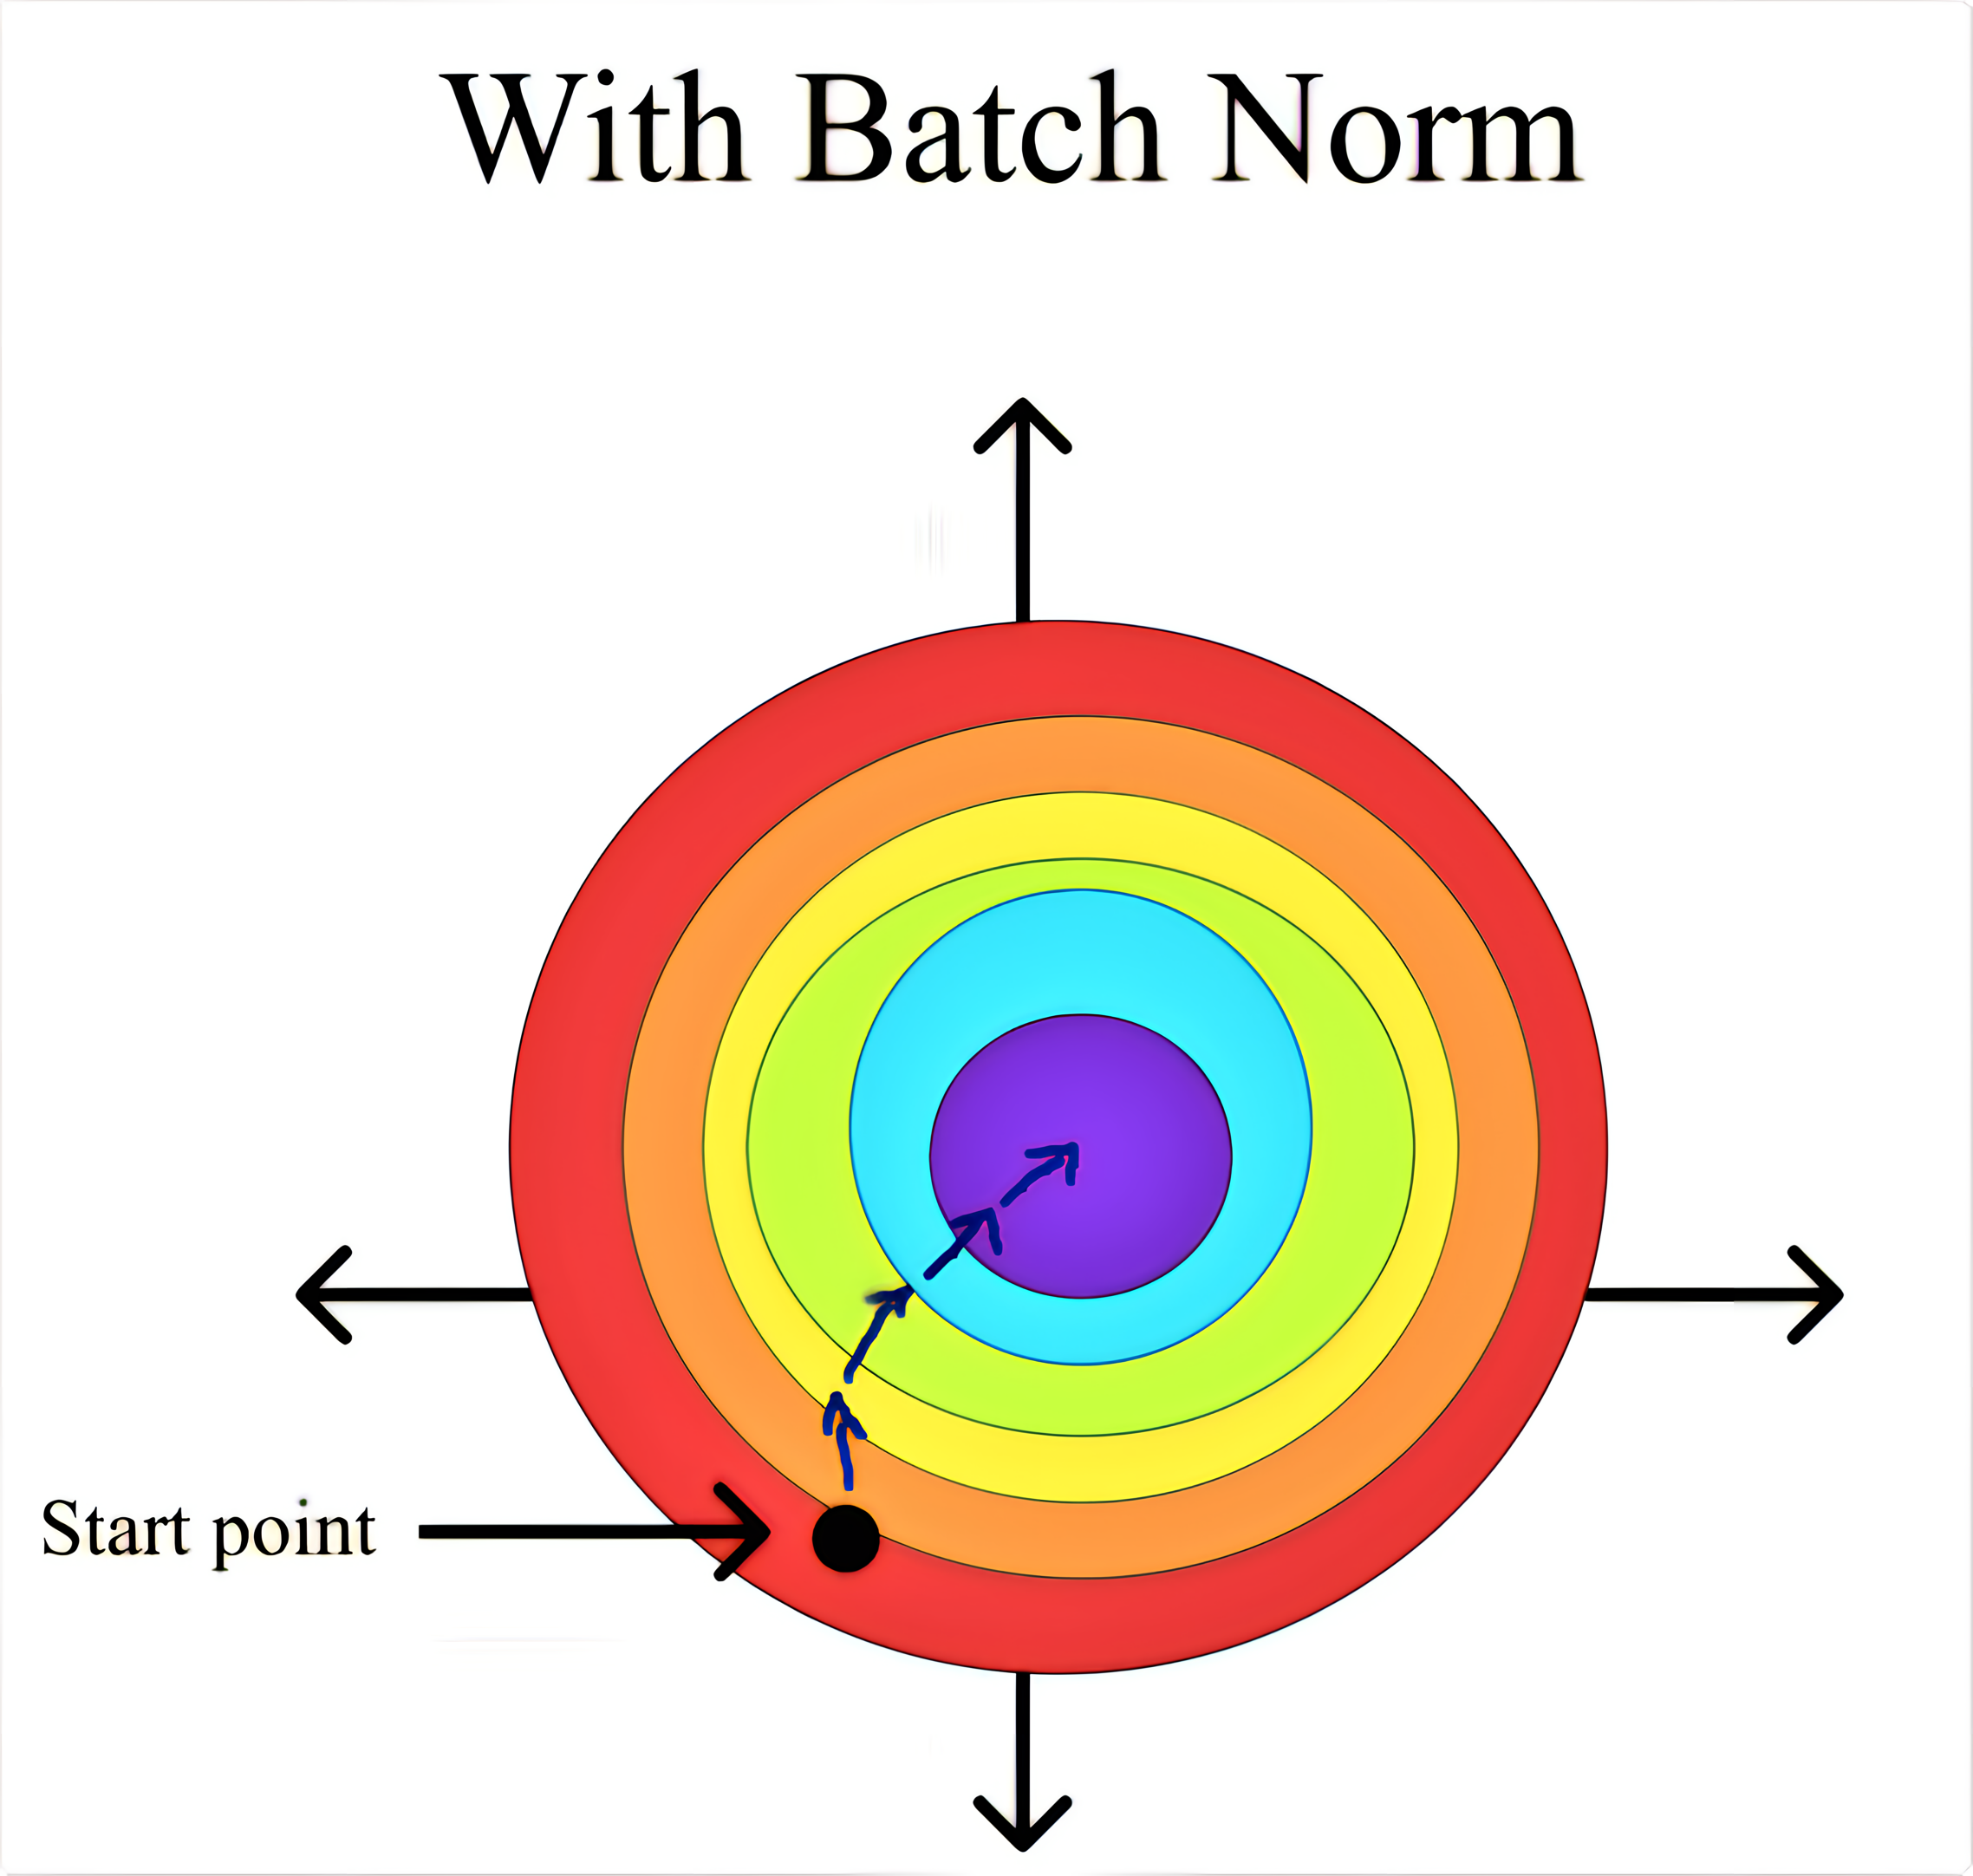
\includegraphics[width=0.3\textwidth]{pic/BN1.png}
            \label{fig:BN_Pros1}
        }
        \subfigure[]{
            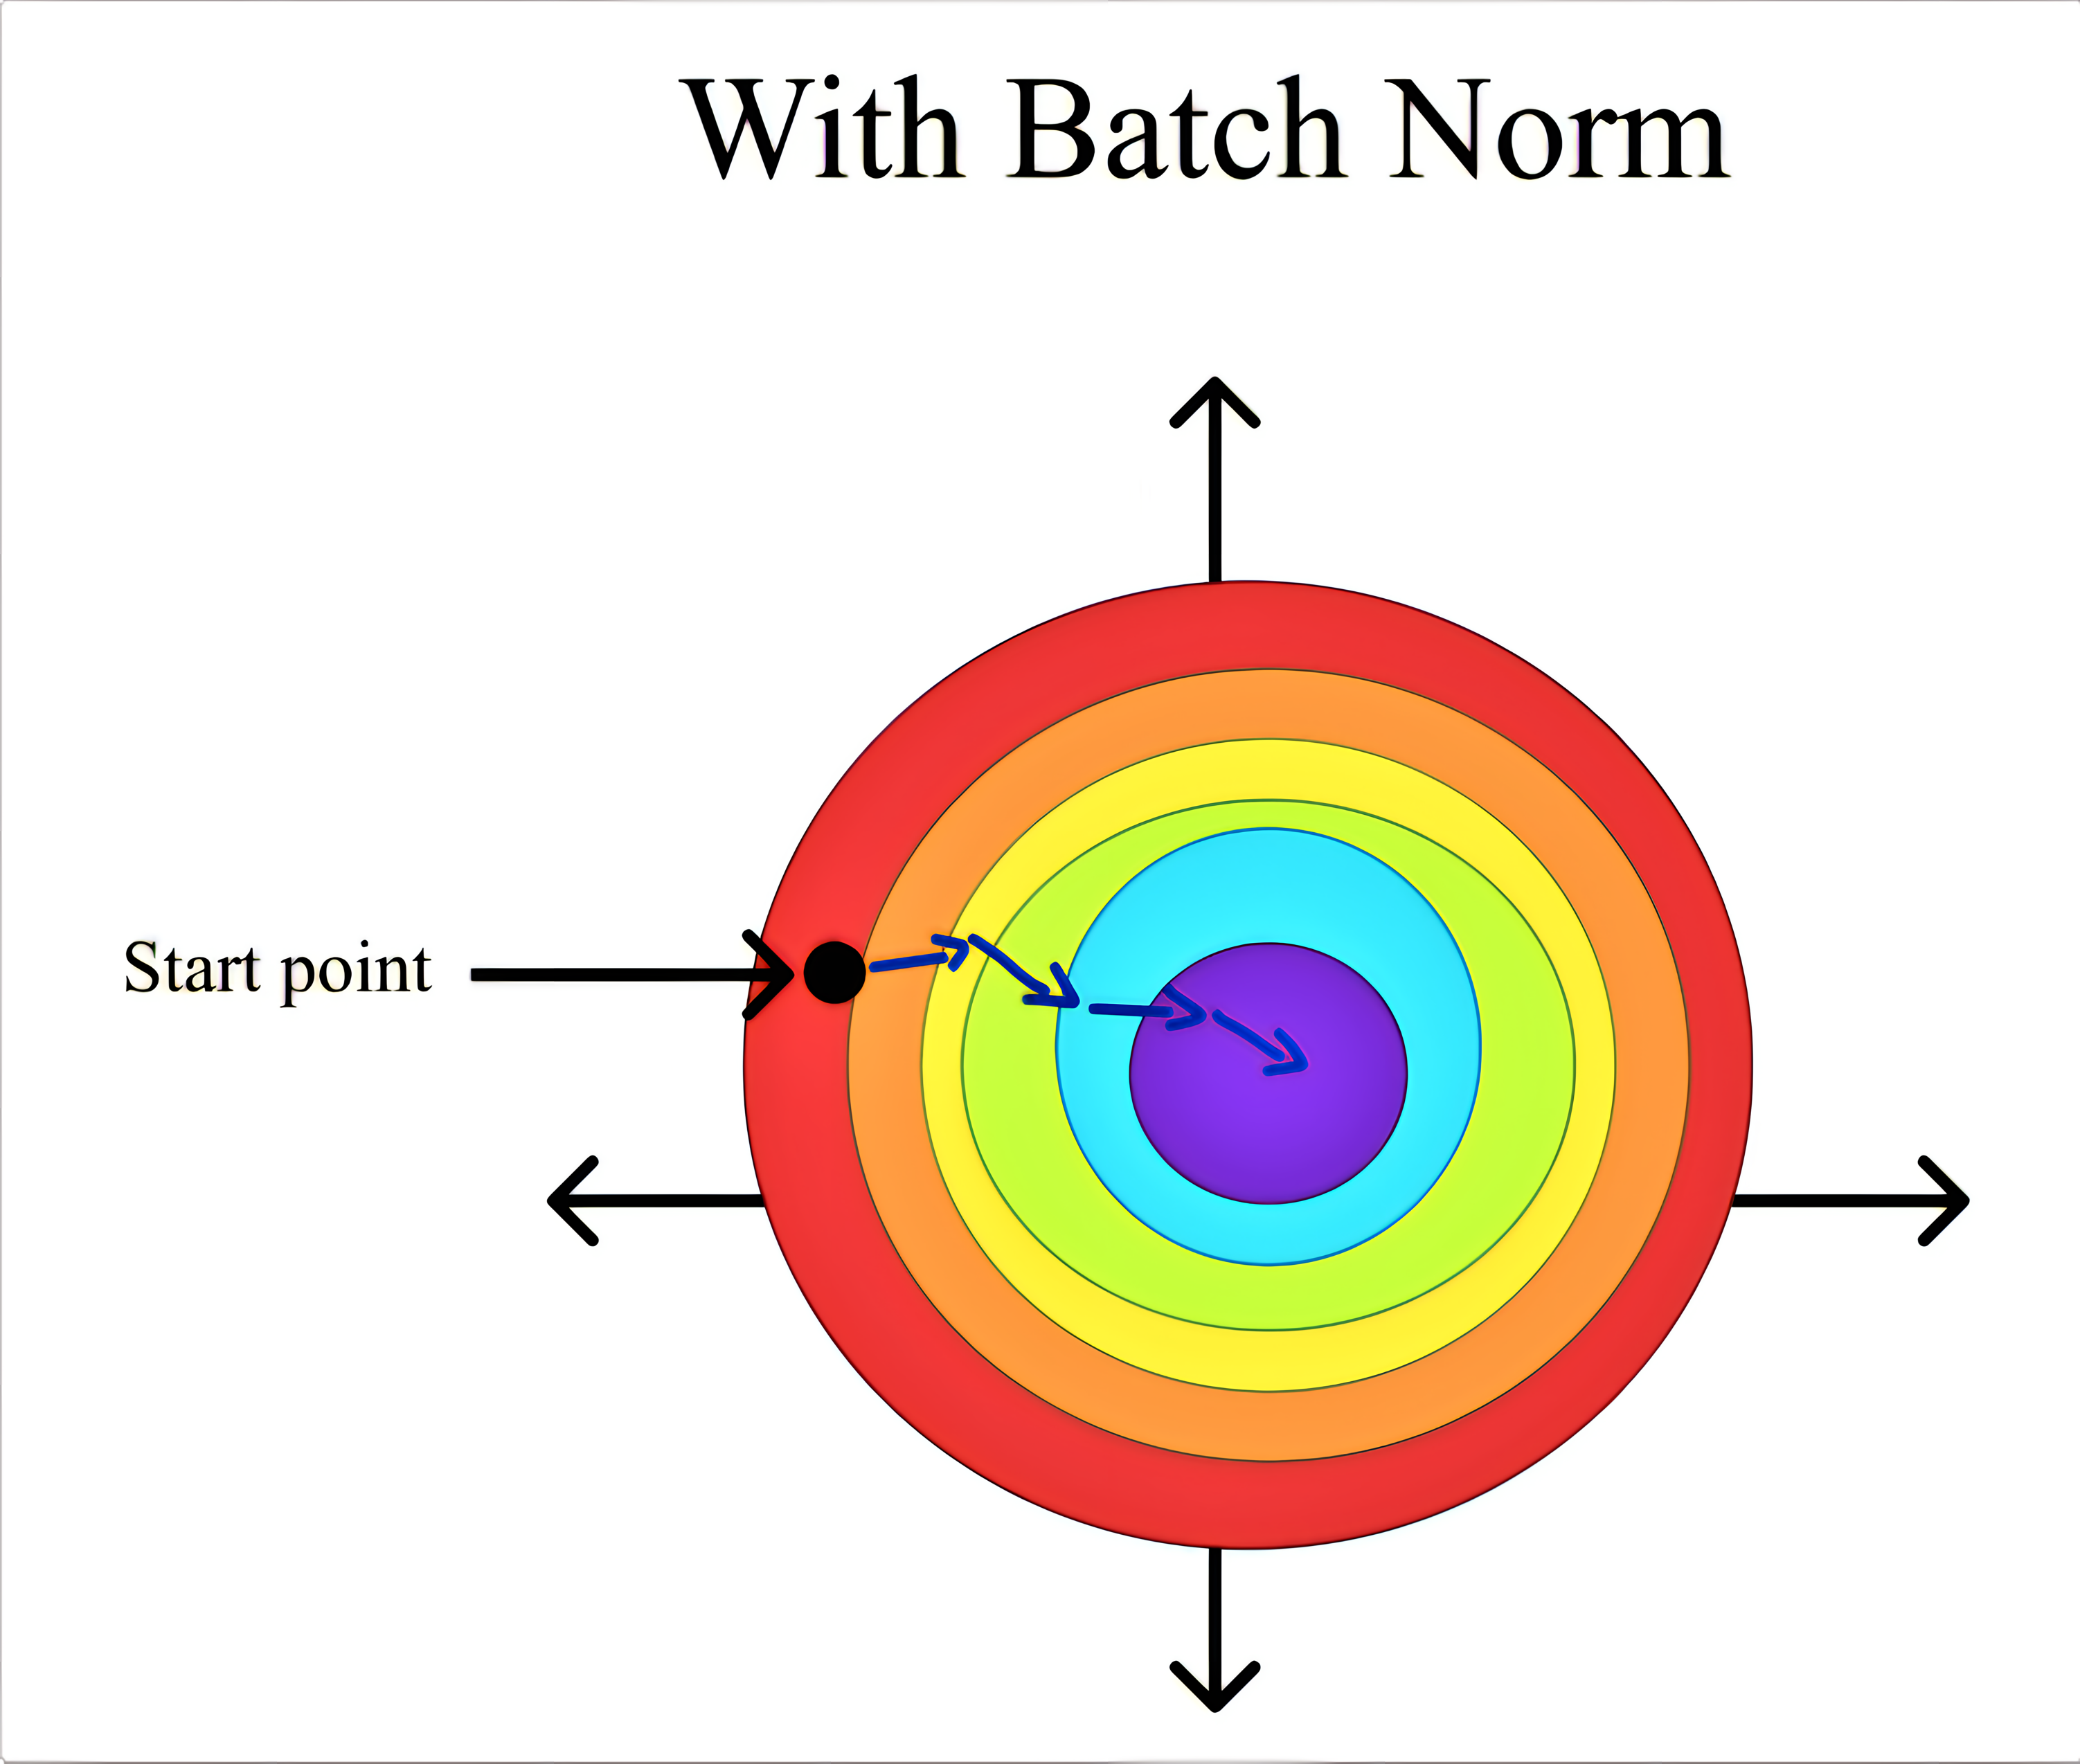
\includegraphics[width=0.33\textwidth]{pic/BN2.png}
            \label{fig:BN_Pros2}
        }
        % \caption{Start point doesn't matter! \href{https://www.linkedin.com/pulse/ways-improve-your-deep-learning-model-batch-adam-albuquerque-lima}{\textcolor{orange}{\textbf{Source}}}}
    \end{figure}

    \vfill
    \begin{tikzpicture}[remember picture,overlay]
        \node[anchor=south west, xshift=0.1cm, yshift=0.22cm] at (current page.south west) {
            \tiny Figure adapted from Gustavo Albuquerque Lima. Ways to Improve Your Deep Learning Model - Batch Normalization and Adam: A Short Course
        };
    \end{tikzpicture}
    
\end{frame}

\begin{frame}{Batch Normalization Pros}

    \textcolor{blue}{\textbf{Why Does Batch Normalization Reduce Sensitivity to Weight Initialization?}}
    \begin{itemize}
        \item Batch normalization smooths the optimization landscape, reducing the dependency on initial weights. 
        \item This allows the model to converge to a minimum efficiently, \textbf{regardless of where optimization begins}.
        


    \end{itemize}
\end{frame}

\begin{frame}{Batch Normalization Cons}

    \textbf{Cons}
    
    \begin{itemize}

        \item \textbf{Batch Size Sensitivity:} Performance may depend on batch size. Very small batches potentially provide unstable statistics.
        \item \textbf{Computational Overhead:} Increases computational-overhead during training.
        \item \textbf{Behavior During Inference:} Switching from batch statistics to moving averages during inference may cause slight discrepancies.

    \end{itemize}
\end{frame}

\subsection{Batch Normalization in Practice}

\begin{frame}{Batch Normalization in Practice}
	
	\textcolor{blue}{\textbf{Where to Apply}}
	
	\begin{itemize}
		\item \textbf{Typical Location:} Apply after the linear transformation (e.g., after a dense layer) and before the activation function.
		\item \textbf{Layer Placement:}
		\newline
		\begin{center}
			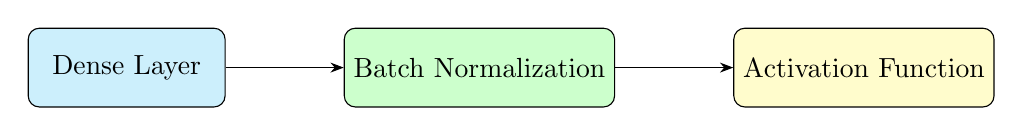
\begin{tikzpicture}[
				node distance=0.9cm and 1.5cm, % Distance between nodes
				every node/.style={draw, rounded corners, text centered, minimum height=1cm, minimum width=2.5cm}, % Style for every node
				bn/.style={fill=green!20}, % Style for batch normalization nodes
				dense/.style={fill=cyan!20}, % New style for dense layer
				act/.style={fill=yellow!20}, % New style for activation functions
				->, >=Stealth % Arrow styles
				]
				
				% Define nodes for the path
				\node[dense] (dense) {Dense Layer};
				\node[bn] (bn1) [right=of dense] {Batch Normalization};
				\node[act] (act1) [right=of bn1] {Activation Function};
				
				% Draw arrows between nodes
				\draw[->] (dense) -- (bn1);
				\draw[->] (bn1) -- (act1);
				
			\end{tikzpicture}
		\end{center}
	\end{itemize}
	
\end{frame}



\subsection{Closing Takeaways on Batch Normalization}

\begin{frame}{Batch Normalization in Practice}
    
    \begin{itemize}

    \item \textbf{Key Point:} Batch normalization stabilizes and accelerates training while offering regularization benefits.
    \item \textbf{Impact on Training:} Facilitates efficient training of deeper networks with less hyperparameter tuning.

\end{itemize}

\end{frame}

\section{MLPs as Universal Approximators}

\begin{frame}{Universal Approximation Theorem}
	\textbf{Key Concept}
	\begin{itemize}
		\item The Universal Approximation Theorem states that a feedforward neural network with:
		\begin{itemize}
			\item A single hidden layer
			\item Sufficient number of hidden neurons
			\item Appropriate activation functions (e.g., sigmoid)
		\end{itemize}
		Can approximate any continuous function on a \textbf{compact subset} of $\mathbb{R}^n$ to any desired accuracy.
	\end{itemize}
	
\end{frame}

\begin{frame}{Understanding Compact Sets}
	\textbf{What is a Compact Set?}
	\begin{itemize}
		\item In the context of the Universal Approximation Theorem, approximation is guaranteed on a \textbf{compact subset} of $\mathbb{R}^n$.
		\item A set is compact if it is both:
		\begin{itemize}
			\item \textbf{Bounded}: Enclosed within a finite space.
			\item \textbf{Closed}: Contains all its boundary points.
		\end{itemize}
		\item Compact sets ensure certain mathematical properties that enable reliable function approximation by the MLP within that region.
	\end{itemize}
\end{frame}

\begin{frame}{Breaking Down Complex Functions}
	\begin{itemize}
		\item Idea: Complex functions can be decomposed into multiple smaller parts, each represented by a simpler function.
		\item By combining a series of simpler functions (like square pulses), the target function can be closely approximated.
	\end{itemize}

		\begin{figure}[h!]
		\centering
		\begin{minipage}{0.43\textwidth}
			\centering
			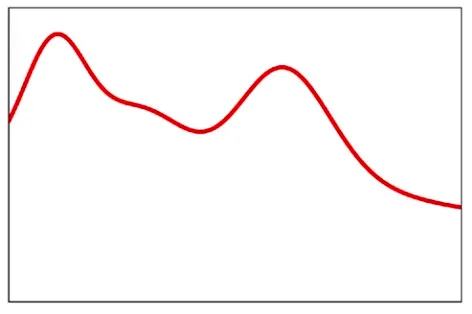
\includegraphics[width=\linewidth]{pic/approximator-1.png}
			\label{fig:fig1}
		\end{minipage} \hfill
		%		\hspace{0.02\textwidth} % Space before the line
		%		\vrule width 0.5pt % Thickness of the line
		%		\hspace{0.02\textwidth} % Space after the line
		\begin{minipage}{0.44\textwidth}
			\centering
			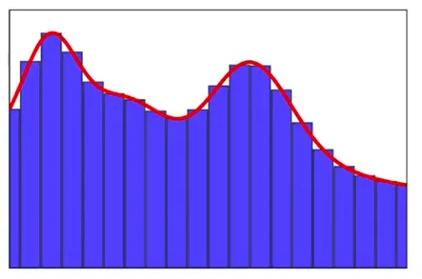
\includegraphics[width=\linewidth]{pic/approximator-2.png}
			\label{fig:fig2}
		\end{minipage}
	\end{figure}
	
	\vfill
	\begin{tikzpicture}[remember picture,overlay]
		\node[anchor=south west, xshift=0.1cm, yshift=0.22cm] at (current page.south west) {
			\tiny Figure adapted from Niranjan Kumar, Illustrative Proof of Universal Approximation Theorem
		};
	\end{tikzpicture}
	
\end{frame}

\begin{frame}{MLPs as Universal Approximators}
	\begin{itemize}
		\item By constructing a series of these \texttt{Square Pulse} functions, we can approximate any continuous function mapping from input to output.
		\item A simple 3-unit MLP with a summing output unit can generate a square pulse.
		\item Therefore, an MLP with enough units and the right configuration is a universal approximator!
		
	\end{itemize}
	
	 \begin{figure}
		        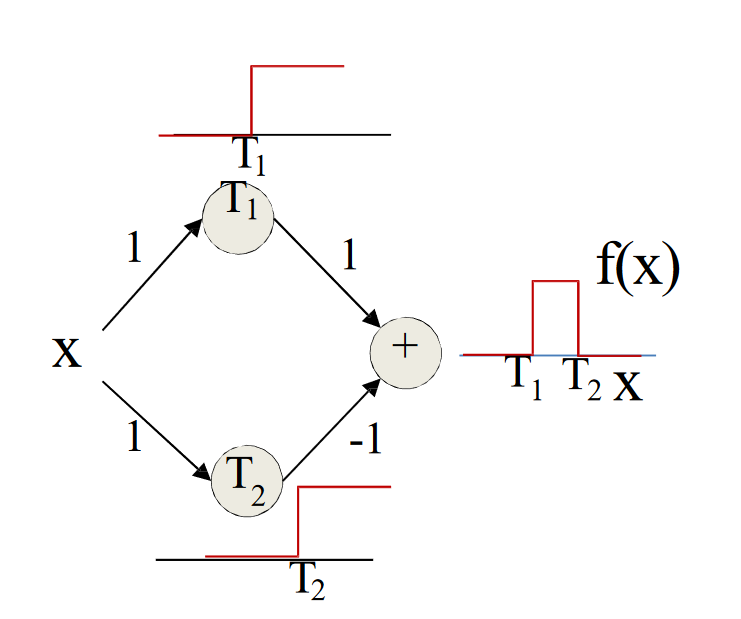
\includegraphics[width=0.38\textwidth]{pic/Puls-Generator.png}
		        \label{fig:puls}
	\end{figure}

	 \vfill
	 \begin{tikzpicture}[remember picture,overlay]
		        \node[anchor=south west, xshift=0.1cm, yshift=0.22cm] at (current page.south west) {
			            \tiny Figure adapted from Dr. Mahdieh Soleymani Baghshah, Deep Learning Course
			        };
	  \end{tikzpicture}
	
\end{frame}

\begin{frame}{Contributions}
	\textbf{These slides are authored by:}
	\begin{itemize}
		\item Faezeh Sarlakifar
		\item Sogand Salehi
	\end{itemize}
	
\end{frame}

\section{References}

\begin{frame}[allowframebreaks]
	\bibliography{ref}
	\bibliographystyle{ieeetr}
	\nocite{*} % used here because no citation happens in slides
	% if there are too many try use:
	% \tiny\bibliographystyle{alpha}
\end{frame}

\begin{frame}
    \begin{center}
        {\Huge Any Questions?}
    \end{center}
\end{frame}

\end{document}